\section{Implementazione}
In questo capitolo verranno illustrati gli strumenti e gli algoritmi utilizzati per l'implementazione del software.

\subsection{Strumenti}
Per lo studio e l'implementazione del \acf{MLBP} è stata creata una libreria in Matlab. 
Matlab (MATrix LABoratory) è un ambiente per il calcolo numerico e l'analisi statistica che comprende anche l'omonimo linguaggio di programmazione creato dalla MathWorks \cite{MATLAB:2013}.

La libreria creata è stata utilizzata in un'applicazione per la rilevazione di errori all'interno di immagini di tessiture.
Per permettere un uso agevole del software e della configurazione dei parametri è stata sviluppata una \acf{GUI}, mostrata in figura \ref{fig:GUI}.

Il codice sorgete di tutta l'applicazione è disponibile sul servizio di versioning Github (\href{http://dining-engineers.github.io/Multi-scale-Local-Binary-Pattern/}{http://dining-engineers.github.io/Multi-scale-Local-Binary-Pattern/}).\\

\begin{figure}[ht]
\begin{center}
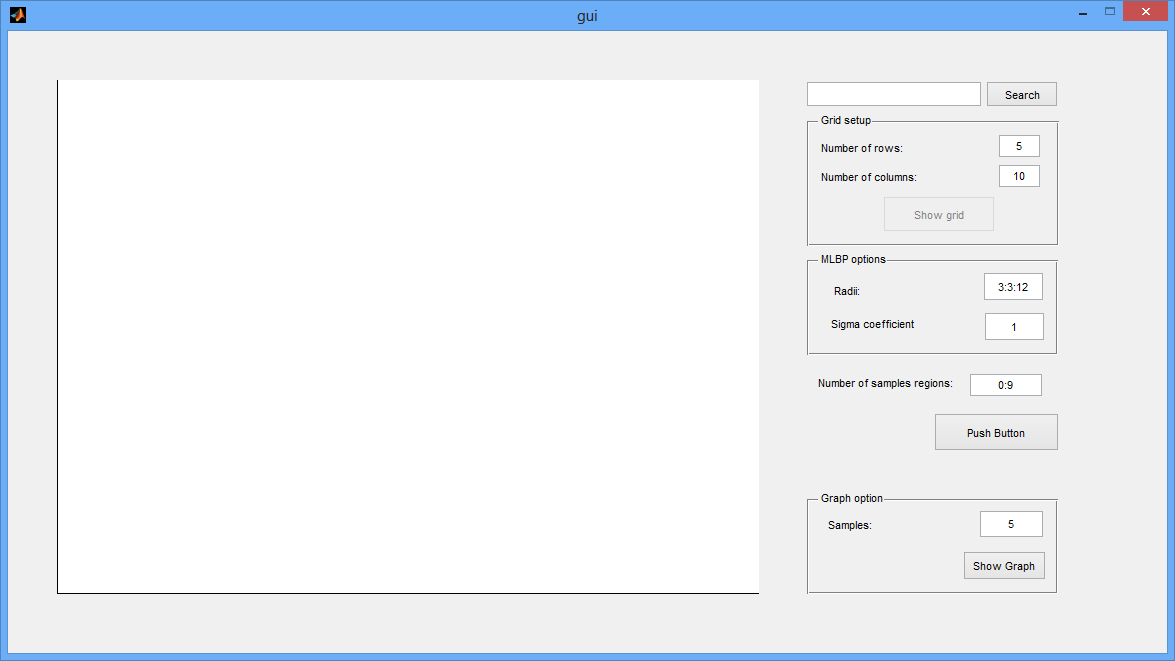
\includegraphics[width=.95\textwidth]{img/gui}
\caption{GUI.}
\label{fig:GUI}
\end{center}
\end{figure}

\subsection{Analisi dell'immagine}
\label{imp:analisi}
Nel contesto della nostra applicazione, le immagini in esame saranno analizzate in scala di grigio.
Per ottenere un descrittore della texture dell'immagine è stata implementata la funzione

\begin{lstlisting}
function [ descriptor ] = getMLBPDescriptor( img, mapping, radii, num_region_rows, num_region_cols, sigma_coefficient )
\end{lstlisting}

che richiede in input: l'immagine da elaborare, la variante di \acs{LBP} da utilizzare (nel nostro caso Uniform LBP), un array contenente i raggi per fare \acs{MLBP}, il numero di righe e colonne in cui l'immagine verrà segmentata ( paragrafo \ref{imp:seg}) ed infine il valore della deviazione standard per l'applicazione del filtro di smoothing gaussiano.

Al suo interno, getMLBPDescriptor(), applica iterativamente all'immagine l'operatore \acs{LBP}.
Ad ogni iterazione $i$, all'immagine viene inizialmente applicato il filtro di smoothing gaussiano

\begin{lstlisting}
% apply gauss smoothing
myfilter = fspecial( 'gaussian', kernel_size, sigma_coefficient );
img = imfilter( img, myfilter, 'replicate' );
\end{lstlisting}

\noindent Successivamente viene chiamata la funzione\cite{lbpcode}

\begin{lstlisting}
function [lbp_img] = lbp( img, radius, num_neighbors, mapping );
\end{lstlisting}

\noindent che calcola l'immagine \acs{LBP} con raggio $radii(i)$, (paragrafo \ref{MLBP:extended}).

\subsubsection{Segmentazione}
\label{imp:seg}
Al fine di determinare le regioni della tessitura in cui sono presenti degli errori, abbiamo deciso di suddividere l'immagine in regioni non sovrapposte. I parametri $num\_region\_rows$ e $num\_region\_cols$ determinano il numero di regioni in cui l'immagine viene suddivisa.
Le regioni sono numerate da $0$ a $num\_region\_rows \cdot num\_region\_cols - 1$.
Le coordinate della k-esima regione sono ottenute attraverso l'utilizzo della funzione

\begin{lstlisting}
function [ rMin, rMax, cMin, cMax ] = gridBounds( imgSize, num_region_rows, num_region_cols, k )
\end{lstlisting}

In figura \ref{fig:GUIpreLBP} viene mostrata la suddivisione in regioni dell'immagine di input. \\

\begin{figure}[ht]
\begin{center}
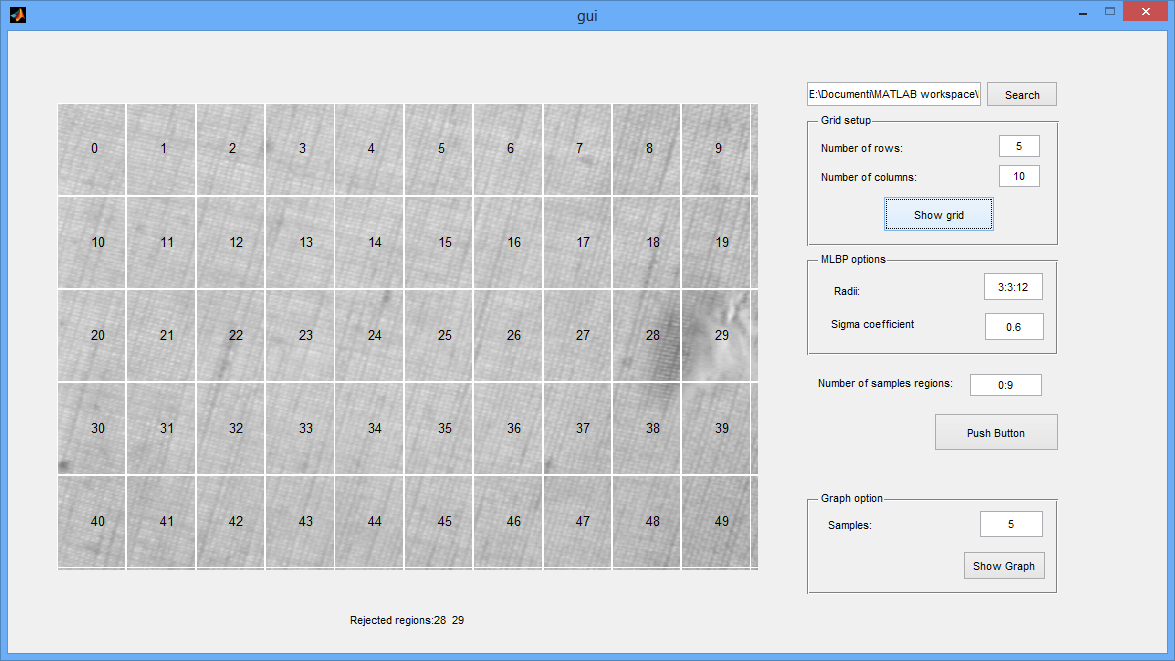
\includegraphics[width=.95\textwidth]{img/gui_pre_lbp}
\caption{ Screenshot della GUI in cui viene mostrata la suddivisione in regioni dell'immagine di input.}
\label{fig:GUIpreLBP}
\end{center}
\end{figure}

In seguito all'operazione di segmentazione dell'immagine, per ogni regione, viene estratto il relativo descrittore \acs{MLBP}:

\begin{equation*}
f = [h_{P, r_{1}}, h_{P, r_{2}}, \cdots, h_{P, r_R}]
\end{equation*}


\noindent come spiegato nel paragrafo \ref{mlbp:desc-mlbp}. 



%	\pagebreak 
%	
%	La costruzione dell'istogramma associato all'LBP di raggio r, $h_{P,r}$ è ottenuta nel modo seguente:
	
%	\begin{lstlisting}
%	M = lbp_image(rMin:rMax, cMin:cMax );
%	% compute histogram of subregion M
%	h = hist(M(:),0:(mapping.num-1));
%	% normalizie histogram
%	h = h/sum(h);
%	\end{lstlisting}



\subsection{Misura di similarità}

Per misurare la similarità tra i descrittori di due regioni $I$ e $J$, possono essere utilizzati vari criteri. Abbiamo implementato le seguenti misure di similarità $Sim(I, J)$:

\begin{itemize}

\item Chi-square criterion:
\begin{equation}
Sim(I, J) = -  \sum_{i} \frac{ (f_{I}(i) - f_{J}(i) )^2}{f_{I}(i) + f_{J}(i)}
\end{equation}

\item Histogram intersection:
\begin{equation}
Sim(I, J) = \sum_{i} \mbox{min}(f_{I}(i),f_{J}(i))
\end{equation}

\item Log-likelihood ratio (Kullack-Leibler 
divergence):
\begin{equation}
Sim(I, J) = - \sum_{i} f_{I}(i)log(f_{J}(i)
\end{equation}

\item Normalize Correlation:
\begin{equation}
Sim(I, J) = \frac{f_{I}f_{J}'}{||f_{I}|| ||f_{J}||}
\end{equation}

\item Normalize Cross-correlation:
\begin{equation}
Sim(I, J) = \frac{\sigma_{f_{I}f_{J}}}{\sigma_{f_{I}}\sigma_{f_{J}}}
\end{equation}


\end{itemize}

\pagebreak
\subsection{Testing}

Lo scopo dell'applicazione è quello di determinare se alcune regioni presentano malformazioni della tessitura al loro interno. Per poter classificare una regione come corretta o errata, è necessario conoscere un certo numero di regioni sicuramente corrette. Come possiamo vedere in figura \ref{fig:GUIpostLBP}, l'utente può specificare nel campo \textit{number of samples regions} il numero delle regioni esatte che vanno a definire il \textit{training set}.

Ogni regione corretta viene confrontata con tutte le altre regioni del training set utilizzando la misura di similarità $Sim(I, J)$, dove  $I$ e $J$ rappresentano i descrittori \acs{MLBP}.
In questo modo si ottengono le misure di similarità del training set da cui possiamo estrarre un valore medio ($\mu_{training}$) ed una deviazione standard ($\sigma_{training}$) che definiscono una distribuzione gaussiana delle misure di similarità delle regioni corrette.

Per classificare una regione $k$, che non appartiene al training set, si confronta il suo descrittore con tutti i descrittori del training set utilizzando la misura di similarità $Sim(I, J)$. In questo modo si ottengono le misure di similarità della regione di test con il training set da cui possiamo estrarre un valore medio ($\mu_{test}$) ed una deviazione standard ($\sigma_{test}$).

La regione $k$ verrà quindi classificata come corretta se \mbox{$ |\mu_{training}- \mu_{test}| \le 3\sigma_{training}$}. Altrimenti verrà classificata come una regione contenente artefatti.
\pagebreak
